\chapter{Analisi e Visualizzazione dei Dati}
\label{cha:Analisi}

Lo scopo di questo capitolo è presentare e discutere i risultati dell’analisi multidimensionale dei dati di affluenza sugli impianti sciistici gestiti da Freccia nel Cielo.
L’analisi è stata condotta mediante l’utilizzo dello strumento di Data Visualization \textbf{Tableau} \cite{Tableau}, che ha permesso di integrare il modello a costellazione dei dati in un ambiente interattivo capace di evidenziare le diverse dimensioni informative rilevanti per lo studio.\\

I risultati sono presentati sotto forma di dashboard analitiche, illustrate nel seguito del capitolo, che supportano l’indagine dei casi di studio individuati.
L’approccio combina tecniche di analisi descrittiva e comparativa, con l’obiettivo di individuare pattern ricorrenti e potenziali trend inaspettati all’interno del dataset.\\

Per strutturare l’esposizione dei risultati in maniera sistematica, l’analisi è stata organizzata attorno a un insieme di domande guida, concepite per enfatizzare gli aspetti più rilevanti dello studio sia per il contesto territoriale di Cortina d’Ampezzo, sia per la società impiantistica considerata.

Ogni domanda è affrontata mediante una o più visualizzazioni, sviluppate utilizzando sia i campi originali del dataset sia campi calcolati dedicati, con lo scopo di fornire risposte chiare e supportate dai dati. Le dashboard presentate includono filtri interattivi, sistemi di selezione, differenti tipologie grafiche e operazioni OLAP\footnote{Tali operazioni, tra cui roll-up, drill-down, slicing e dicing, sono state discusse nei capitoli precedenti.}, garantendo un’esplorazione dinamica ed esaustiva delle informazioni disponibili.\\

Le principali domande a cui si intende rispondere sono:

\begin{enumerate}
    \item \textbf{Analisi 1 – Picchi di affluenza stagionale}~(\ref{sec:analisi1}):  
    In quali periodi della stagione invernale si registrano i massimi livelli di affluenza agli impianti, e come si distribuiscono i picchi di passaggi in corrispondenza dei diversi periodi festivi (Natale, Carnevale, ordinario)?

    \item \textbf{Analisi 2 – Variazioni settimanali e pattern giornalieri}~(\ref{sec:analisi2}):  
    Quali variazioni si osservano nei livelli di affluenza tra i diversi giorni della settimana, in particolare tra venerdì, sabato e domenica, e quali tendenze emergono nel confronto cumulativo dei passaggi?

    \item \textbf{Analisi 3 – Classificazione e influenza delle condizioni meteorologiche}~(\ref{sec:analisi3}):  
    In che modo le condizioni atmosferiche, e in particolare la temperatura percepita e l’escursione termica giornaliera, caratterizzano l’andamento della stagione sciistica e la distribuzione delle giornate nelle diverse categorie termiche?

    \item \textbf{Analisi 4 – Impatto delle giornate nevose sulle tipologie di skipass}~(\ref{sec:analisi4}):  
    Qual è l’effetto delle giornate con precipitazioni nevose sull’affluenza complessiva e sull’utilizzo delle diverse tipologie di skipass (Valle e Dolomiti Superski), e come varia tale impatto nel corso della stagione?
\end{enumerate}


Le sezioni seguenti approfondiscono ciascuna di queste domande, presentando le dashboard costruite e i relativi indicatori calcolati, accompagnati da un commento interpretativo volto a evidenziare le tendenze emerse e la loro rilevanza per la gestione turistica e operativa della località.

\newpage

%-----------------------------------------
\section{Campi calcolati e parametri su Tableau}

Prima di procedere all’analisi delle domande chiave, è opportuno evidenziare che, per supportare la lettura e l’interpretazione dei dati, nell’ambiente Tableau sono stati sviluppati diversi parametri e campi calcolati. Tali componenti hanno contribuito a migliorare la chiarezza delle visualizzazioni e l’efficacia analitica delle dashboard.

Nel seguito vengono illustrati alcuni tra i principali campi calcolati adottati; ulteriori elementi non esplicitamente descritti in questa sezione saranno comunque richiamati, ove necessario, durante l’analisi dei grafici.\footnote{La lista completa dei campi calcolati è riportata negll'appendice.}



\subsection*{Classificazione Periodo Festivo}
Di seguito viene presentato il campo calcolato che permette la distinzione del periodo festivo nel corso della stagione, grazie a un range di date fissato.

\begin{lstlisting}[language=SQL, caption={Campo calcolato: Classificazione periodo festivo}]
IF [Data] >= DATE("2023-12-24") AND [Data] <= DATE("2024-01-06") THEN "Natale"
ELSEIF [Data] >= DATE("2024-02-08") AND [Data] <= DATE("2024-02-17") THEN "Carnevale"
ELSE "Ordinario"
END
\end{lstlisting}

Questo campo consente di identificare e visualizzare i principali periodi festivi della stagione invernale, tipicamente associati a un aumento dell’affluenza agli impianti sciistici. La classificazione è applicata a tutte le stagioni analizzate, adattando gli intervalli temporali in base al calendario di ciascun anno.\\

In particolare, il periodo di \textbf{Carnevale} non presenta date fisse e viene quindi delimitato considerando il Giovedì Grasso come data di inizio e il weekend del Carnevale Ambrosiano come data conclusiva. Tale scelta riflette le differenze territoriali nelle festività, che possono influenzare i flussi turistici e le decisioni di viaggio degli utenti provenienti da diverse aree geografiche.\\

Il periodo \textbf{Natalizio}, invece, presenta una maggiore stabilità temporale: esso decorre convenzionalmente dal 24 dicembre fino al 6 gennaio, con una possibile estensione di uno o due giorni in funzione della collocazione dell’ultimo weekend festivo della stagione. Questa delimitazione consente di catturare in modo più realistico le dinamiche turistiche legate alle festività di fine anno, tradizionalmente caratterizzate da un afflusso particolarmente elevato.

\subsection*{Classificazione Categoria Temperatura} \label{subsec:Cat_temperatura}
Un ulteriore gruppo di campi calcolati è stato sviluppato per classificare le giornate in base alla temperatura percepita sulle piste da sci. Tale classificazione consente di valutare l'effetto congiunto della temperatura e del vento, fattori che incidono direttamente sul comfort degli utenti e potenzialmente sulla loro propensione a frequentare gli impianti.

Il primo campo necessario definisce la temperatura base, ovvero il valore termico utilizzato come riferimento per l’analisi. Questo campo agisce come selettore e consente di scegliere tra le temperature minima e media, escludendo la temperatura massima in quanto raramente rappresentativa delle condizioni percepite dagli sciatori durante la giornata, risultando quindi poco significativa ai fini dell’analisi.
Il valore predefinito è impostato sulla temperatura media, in quanto più indicativa dell’intervallo orario in cui gli impianti sono operativi e dell’esperienza termica complessiva sulle piste.\\

A partire dalla temperatura base , viene calcolata la \textbf{Temperatura Percepita}, integrando l'effetto del vento, se la sua velocità è maggiore di una certa soglia, mediante l'applicazione di una formula riconducibile all'indice \textbf{Wind Chill}, che consente di stimale la diminuizione della percezione della temperatura in presenza di forte ventilazione.\\

Infine sulla base della temperatura percepita viene generato il campo \textbf{Categoria Temperatura} presentato di seguito, che classifica ciascuna giornata in fasce qualitative (ad es. Freddo, Mite, Caldo). Questa categorizzazione favorisce un’interpretazione immediata delle condizioni climatiche delle giornate e permette di analizzarne l’impatto potenziale sui flussi di utenza.
Si noti che anche in questo campo è presente un controllo sull'intensità del vento, questo per considerare alcuni casi in cui, pur non verificandosi pienamente le condizioni per l'applicazione formale dell'indice, la presenza di vento sostenuto determini comunque una percezione soggettiva più rigida.\\


\begin{lstlisting}[language=SQL, caption={Campo calcolato: Categoria Temperatura}]
IF ISNULL([Temp Percepita]) THEN
    "Missing"
ELSEIF [Temp Percepita] < 2 THEN
    "Freddo"
ELSEIF [Temp Percepita] <= 8 
   AND [Velocita vento  (m/s)] >= 4 THEN
    "Freddo"
ELSEIF [Temp Percepita] <= 12 THEN
    "Mite"
ELSE
    "Caldo"
END
\end{lstlisting}

Si evidenzia che i campi calcolati \textbf{Temperatura Base} e \textbf{Temperatura Percepita} sono riportati integralmente in Appendice ai seguenti riferimento \ref{appendix:Temp_Base}. 

\subsection*{Parametri}

Oltre ai campi calcolati, Tableau consente di definire dei \textbf{parametri}, ovvero elementi dinamici che fungono da selettori di valore e permettono di rendere interattive le visualizzazioni.  
Un parametro può assumere uno o più valori predefiniti, di cui uno è impostato come valore di default visualizzato all’apertura della dashboard.  
La modifica del parametro da parte dell’utente comporta l’aggiornamento immediato dei grafici e dei campi calcolati collegati, consentendo così una lettura flessibile e personalizzabile dei dati.

Di seguito sono riportati i principali parametri utilizzati nelle dashboard:

\begin{itemize}
    \item \textbf{Selezione Skipass}: consente di scegliere la tipologia di skipass da utilizzare nei calcoli relativi ai passaggi.  
    I valori disponibili sono: All (tutti i titoli), DS (Dolomiti Superski) e Valle (skipass locale).  
    La selezione del parametro influisce su tutte le viste collegate, aggiornando dinamicamente le misure e i grafici.
    
    \item \textbf{Tipo Temperatura}: determina quale valore termico viene impiegato nei campi calcolati meteorologici, permettendo di scegliere tra la temperatura minima e la temperatura media.  
    Questa opzione consente di confrontare le diverse metodologie di calcolo della temperatura percepita, valutandone l’impatto sulle analisi climatiche e di affluenza.
\end{itemize}

nel seguito vengono presentate le analisi condotte sulla base delle domande guida elencate all'inizio di questo capitolo.


%-----------------------------------------
\section{Analisi 1 – Picchi di affluenza stagionale}\label{sec:analisi1}

La prima analisi condotta ha l’obiettivo di individuare i periodi della stagione sciistica caratterizzati dai livelli più elevati di affluenza. Tale indagine costituisce il punto di partenza naturale dello studio, poiché la periodizzazione degli accessi rappresenta una variabile chiave che influenzerà anche le analisi successive, in particolare per quanto riguarda le festività e i flussi turistici associati.\\

Per rispondere a questa domanda è stata realizzata una \textbf{dashboard} che mostra l’andamento dei \textbf{passaggi totali giornalieri} registrati su tutti gli impianti del comprensorio \textit{Freccia nel Cielo} nel corso della stagione 2023–24.  
La vista principale consente di individuare visivamente i picchi di affluenza e di distinguere i periodi festivi grazie all’applicazione del campo calcolato “\textbf{Periodo Festivo}”, descritto in precedenza, che assegna una colorazione diversa alle giornate appartenenti alle festività di \textbf{Natale} e \textbf{Carnevale}, uniche rilevanti per l’arco stagionale considerato.\\

La vista secondaria, invece, mostra il \textbf{cumulativo dei passaggi} per ciascun periodo festivo, consentendo un confronto immediato tra le tre categorie considerate (Ordinario, Natale, Carnevale).  
Di seguito è riportata la visualizzazione complessiva nella figura~\ref{fig:passaggi_tot_stagione}.



%Grafico qui
\begin{figure}[htbp]
    \centering
    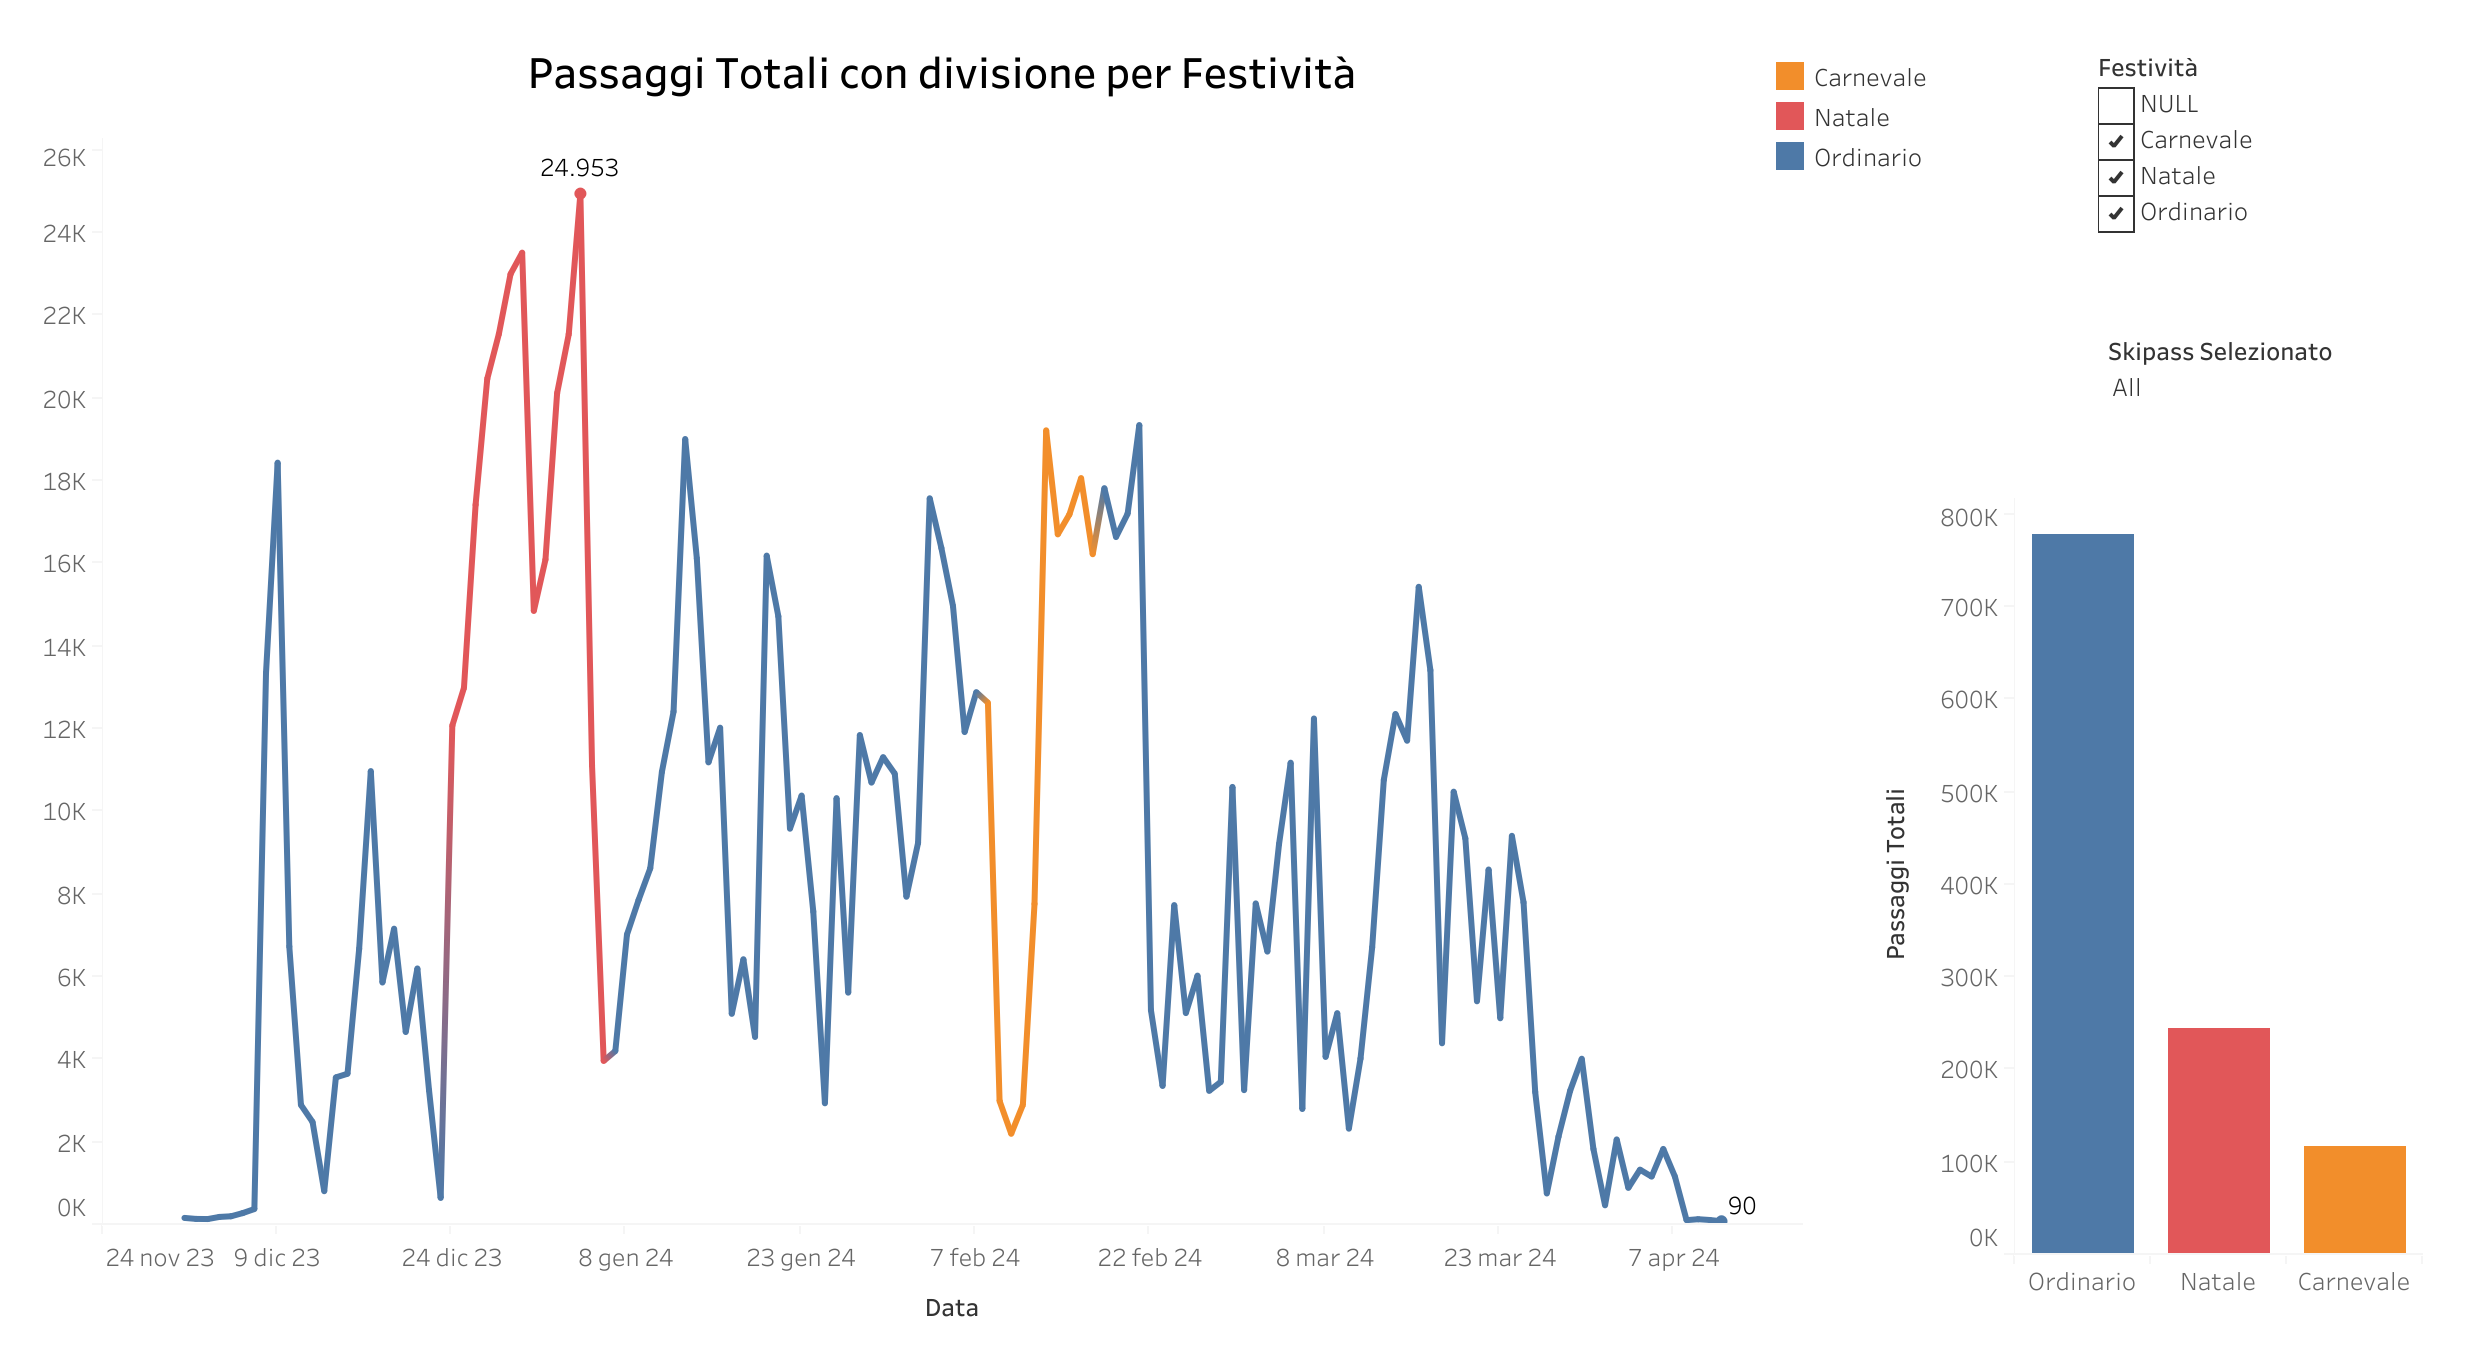
\includegraphics[width=0.95\textwidth]{images/Tableau/Studio_1/Passaggi Totali.png}
    \caption{Andamento giornaliero dei passaggi totali nella stagione 2023–24, suddivisi per periodo festivo.}
    \label{fig:passaggi_tot_stagione}
\end{figure}



Per ampliare la lettura temporale dei dati è stata inoltre introdotta una vista alternativa che applica un’operazione di \textbf{Roll-Up} sulla dimensione temporale, aggregando i dati a livello \textbf{settimanale}.  
Questa trasformazione consente di valutare l’evoluzione dei flussi in un periodo di tempo più ampio e di cogliere con maggiore chiarezza gli effetti successivi alle festività.  
La figura~\ref{fig:passaggi_tot_settimana} mostra l’andamento settimanale dei passaggi totali, evidenziando i trend di continuità e di ripresa post-festiva.


\paragraph{Struttura della visualizzazione e variabili impiegate}
\begin{itemize}
    \item \textbf{Asse X}: Nella vista principale rappresenta la Data, con possibile operazione di Roll-up lungo la gerarchia per aumentare la granularità (giorno \textrightarrow  settimana \textrightarrow  mese); nella vista secondaria riporta invece le tre tipologie di periodo festivo.
    \item \textbf{Asse Y}:  per entrambe le viste è costituito dai \textbf{passaggi totali}, calcolati sul totale o filtrati in base alla tipologia di skipass selezionata tramite il parametro \textbf{Skipass Selezionato}, che consente di visualizzare i dati complessivi (All) o solo quelli relativi ai titoli  “ di Valle” e “Dolomiti Superski”, il tutto è incluso nel campo calcolato \textbf{Tipo SKipass} presente nell'appendice \ref{appendix:tipo_skipass}.
    \item \textbf{Filtri e colorazione}: Campo calcolato “Periodo Festivo”, utilizzato per evidenziare e confrontare i diversi intervalli stagionali.
    \item \textbf{Tipologia di Grafico}: lineare nella visualizzazione principale e a barre nella visualizzazione secondaria.
\end{itemize}

\paragraph{Valutazioni e osservazioni}
Dall’analisi emerge chiaramente come il \textbf{periodo natalizio} rappresenti il picco assoluto di affluenza, con il massimo registrato il \textbf{4 gennaio} (\textbf{24.953 passaggi}) (vedi \ref{fig:spec_giorno} per la specifica del giorno), in linea con le aspettative relative ai flussi turistici della località. \\

Un elemento rilevante che si può cogliere a vista d'occhio nell'analisi è relativo alla fase natalizia, che mostra un andamento fortementente \textbf{irregolare}, caratterizzato da forti oscillazioni giornaliere tra picchi molto elevati e giornate di affluenza più contenuta.
Il periodo carnevalesco, al contrario, evidenzia un comportamento più \textbf{stabile e uniforme}, mantenendo valori di affluenza alti anche nei giorni immediatamente successivi alla fine della festività.  
La media giornaliera dei passaggi tra il 13 e il 21 febbraio si attesta su circa \textbf{17.600 passaggi}, un valore molto vicino alla media registrata tra il 25 dicembre e il 6 gennaio (\textbf{17.800 passaggi}), ma con una variabilità sensibilmente inferiore.  
Ciò suggerisce una presenza turistica più regolare e distribuita nel tempo, probabilmente favorita dalla concomitanza di vacanze scolastiche e da condizioni meteorologiche più prevedibili rispetto al periodo natalizio; tramite il filtro sui periodi festivi inoltre è possibile visionare la dashboard in appendice \ref{fig:passaggi_tot_noNatale} con l'esclusione del periodo natalizio per avere un  confronto senza i picchi natalizi.

La visualizzazione con roll-up settimanale (\ref{fig:passaggi_tot_settimana}) conferma e rafforza questa lettura: la settimana centrale di Natale rappresenta il picco assoluto stagionale (\textbf{133.838 passaggi}), seguita da un progressivo calo e da una successiva ripresa durante il Carnevale.  
Dopo quest’ultimo periodo, l’andamento mostra una discesa più graduale ma costante, evidenziando come l’affluenza rimanga sostenuta anche nelle settimane successive, probabilmente grazie a condizioni di innevamento ancora favorevoli.\\

In sintesi, l’analisi mostra come il periodo natalizio, pur rimanendo il momento di massima affluenza, presenti un andamento più volatile, mentre il Carnevale rappresenta una fase di equilibrio e continuità per l’affluenza stagionale.  
Queste evidenze risultano particolarmente utili ai fini gestionali, poiché permettono di pianificare in modo differenziato le risorse e le strategie operative in funzione delle diverse dinamiche festive.

%-----------------------------------------
\section{Analisi 2 – Variazioni settimanali e pattern giornalieri}
\label{sec:analisi2}

La seconda analisi ha l'obiettivo di individuare quali giorni della settimana registrano i livelli più elevati di affluenza agli impianti. Tale valutazione risulta utile al fine di pianificare in modo più efficiente le attività operative, l'organizzazione del personale e la gestione delle risorse nelle giornate caratterizzate da maggiore pressione turistica. Questa analisi è presentata tramite una Dashboard contenente due visualizzazioni distinte.\\

 La prima analizza i \textbf{passaggi totali nei vari giorni settimanali}. Per non andare a sovraccaricare i grafici di troppe variabili, si è scelto di presentare i dati dei giorni più rilevanti in questa sezione, quindi quelle relativo ai giorni del fine settimana, confrontando \textbf{venerdì, sabato e domenica}. Questa scelta è motivata dal fatto che il weekend rappresenta, indipendentemente dalle festività, il periodo di picco ricorrente dell’affluenza turistica.

Il secondo grafico riporta invece il \textbf{totale cumulativo dei passaggi per giorno della settimana}, consentendo di valutare l’incidenza complessiva di ciascun giorno sul totale stagionale e di stimare quali giornate richiedano una maggiore capacità organizzativa.

 Di seguito in  \ref{fig:Weekend_cumulativo}  è presentata la dashboard complessiva che permette quindi una interpretazione  interattiva dei dati, grazie al filtro modificabile \textbf{Giorni selezionati}, secondo due metodologie di rappresentazione distinte ma collegate tra loro.



\begin{figure}[htbp]
    \centering
    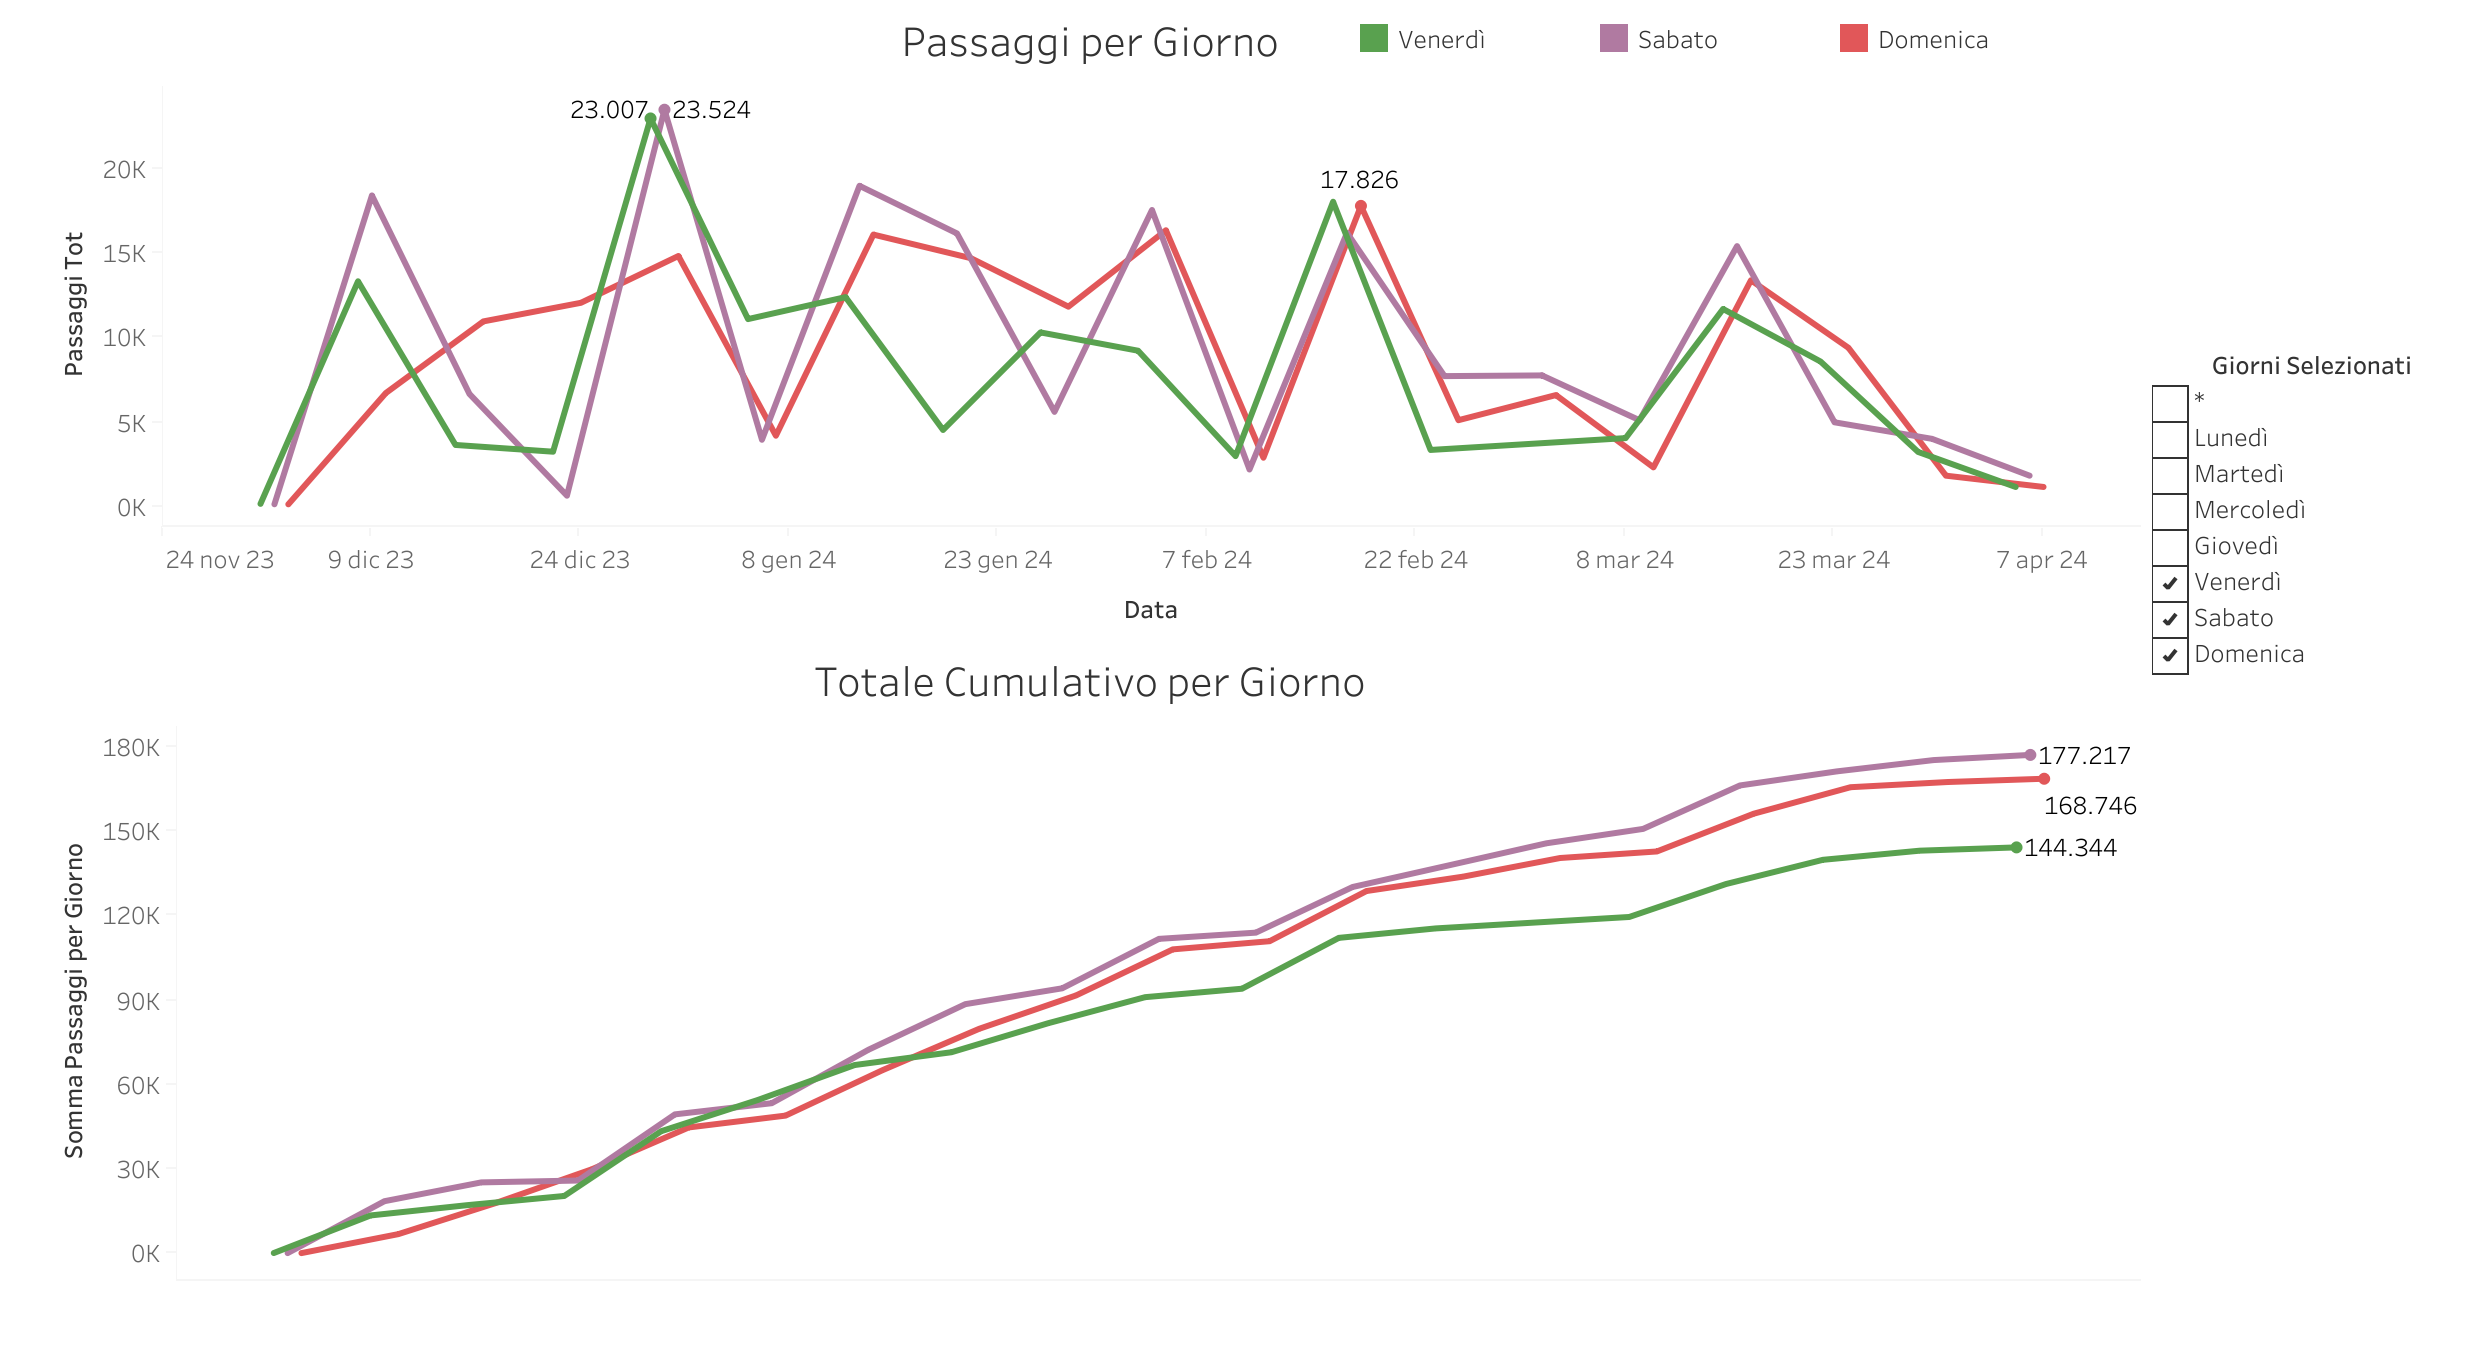
\includegraphics[width=0.95\textwidth]{images/Tableau/Studio_2/Dash_Weekend_cumulativo.png}
    \caption{Dashboard per passaggi settimanali con totale cumulativo}
    \label{fig:Weekend_cumulativo}
\end{figure}

%grafici

\paragraph{Struttura della visualizzazione e variabili Impiegate}
\begin{itemize}
    \item \textbf{Asse X}: Data (variabile continua).
    \item \textbf{Asse Y}: Passaggi totali (variabile continua); nel secondo grafico è riportato il totale corrente, calcolato come somma cumulativa dei passaggi per giorno mediante la funzione di aggregazione “Totale corrente”.
    \item \textbf{Filtri e colorazioni}:differenziazione dei giorni mediante codici colore distinti; filtro interattivo sui giorni selezionati, estendibile a tutti i giorni della settimana tramite variabili testuali.
    \item \textbf{Tipologie di grafico}: grafici lineari multipli.
\end{itemize}


\paragraph{Valutazioni e osservazioni}
Dall’analisi emerge un risultato particolarmente rilevante e, in parte, inatteso: il giorno con il maggior numero di passaggi registrati durante la stagione è il \textbf{sabato}, non solo, se si va ad analizzare il weekend si nota che la linea del sabato è in generale sempre la più alta.
Si potrebbe infatti presumere che la giornata di picco corrisponda alla \textbf{domenica}, quando le presenze turistiche raggiungono generalmente i livelli massimi. Tuttavia, nel caso di Cortina d’Ampezzo, la dinamica appare differente.
Una spiegazione di questo fenomeno può essere trovata nella conformazione geografica della valle ampezzana, che si estende come una conca chiusa avendo un'unica strada principale ad esclusione dei passi, su cui si distribuisce il traffico, induce molti visitatori a lasciare la località la domenica, preferendo rientrare anticipatamente per evitare il traffico del rientro.
Ne risulta dunque un picco di presenze nella giornata di sabato, seguito da una progressiva diminuzione dei passaggi la domenica.\\

Un ulteriore elemento interessante emerge osservando il \textbf{grafico cumulativo}: includendo gli altri giorni della settimana, si nota che, dopo il sabato, il secondo giorno con il più alto totale di passaggi non è la domenica, bensì il \textbf{martedì}.
Questo andamento, apparentemente controintuitivo, suggerisce una ripresa significativa delle attività subito dopo il lunedì, probabilmente legata a turisti in vacanza prolungata, nuove partenze settimanali e posizionameni delle festività nel calendario.
Si tratta di un’informazione di rilievo per la gestione operativa degli impianti, che possono pianificare in modo più efficiente la distribuzione delle risorse durante la settimana.

La versione estesa della dashboard, con l'ulteriore selezione del martedì, è riportata in Appendice al riferimento~\ref{fig:dash_tuesday}.


%-----------------------------------------

\section{Analisi 3 – classificazione e influenza delle Condizioni metereologiche}
\label{sec:analisi3}

Questa analisi è stata sviluppata per confrontare le condizioni meteorologiche osservate durante l’intera stagione invernale, con l’obiettivo di classificare ciascuna giornata secondo le tre categorie di temperatura definite nella sezione~\ref{subsec:Cat_temperatura}: \textbf{freddo}, \textbf{mite} e \textbf{caldo}.  \\

Nella vista principale, ogni giornata è rappresentata da una barra la cui colorazione identifica la categoria di temperatura percepita .  
L’altezza della barra è determinata da un parametro denominato \textbf{Range Size}, calcolato come la differenza tra la temperatura massima e quella minima registrata nella stessa giornata, e rappresentante quindi l’\textbf{escursione termica giornaliera}.  
Sovrapposta alle barre è tracciata una linea grigia che mostra l’andamento della \textbf{temperatura percepita} nel corso dell'intera stagione, ottenuta mediante il campo calcolato descritto in appendice~\ref{}.  
Questa combinazione a doppio asse consente di osservare simultaneamente sia la variabilità giornaliera delle temperature sia l’andamento generale percepito nel corso della stagione. \\

La vista secondaria, collocata sulla destra della dashboard, riassume invece i \textbf{passaggi totali ai tornelli} in funzione della categoria di temperatura.  
Essa consente di valutare in modo sintetico la distribuzione complessiva dell’affluenza in relazione alle diverse condizioni termiche: i valori più elevati si registrano nelle giornate classificate come “fredde”, seguite da quelle “miti”, mentre le giornate “calde” mostrano un’incidenza pressoché marginale.  
Questa rappresentazione, quindi, fornisce un quadro immediato dell’impatto delle condizioni climatiche sull’utilizzo degli impianti e permette di collegare i pattern meteorologici osservati nel grafico principale con i comportamenti di affluenza.


%grafico

\begin{figure}[htbp]
    \centering
    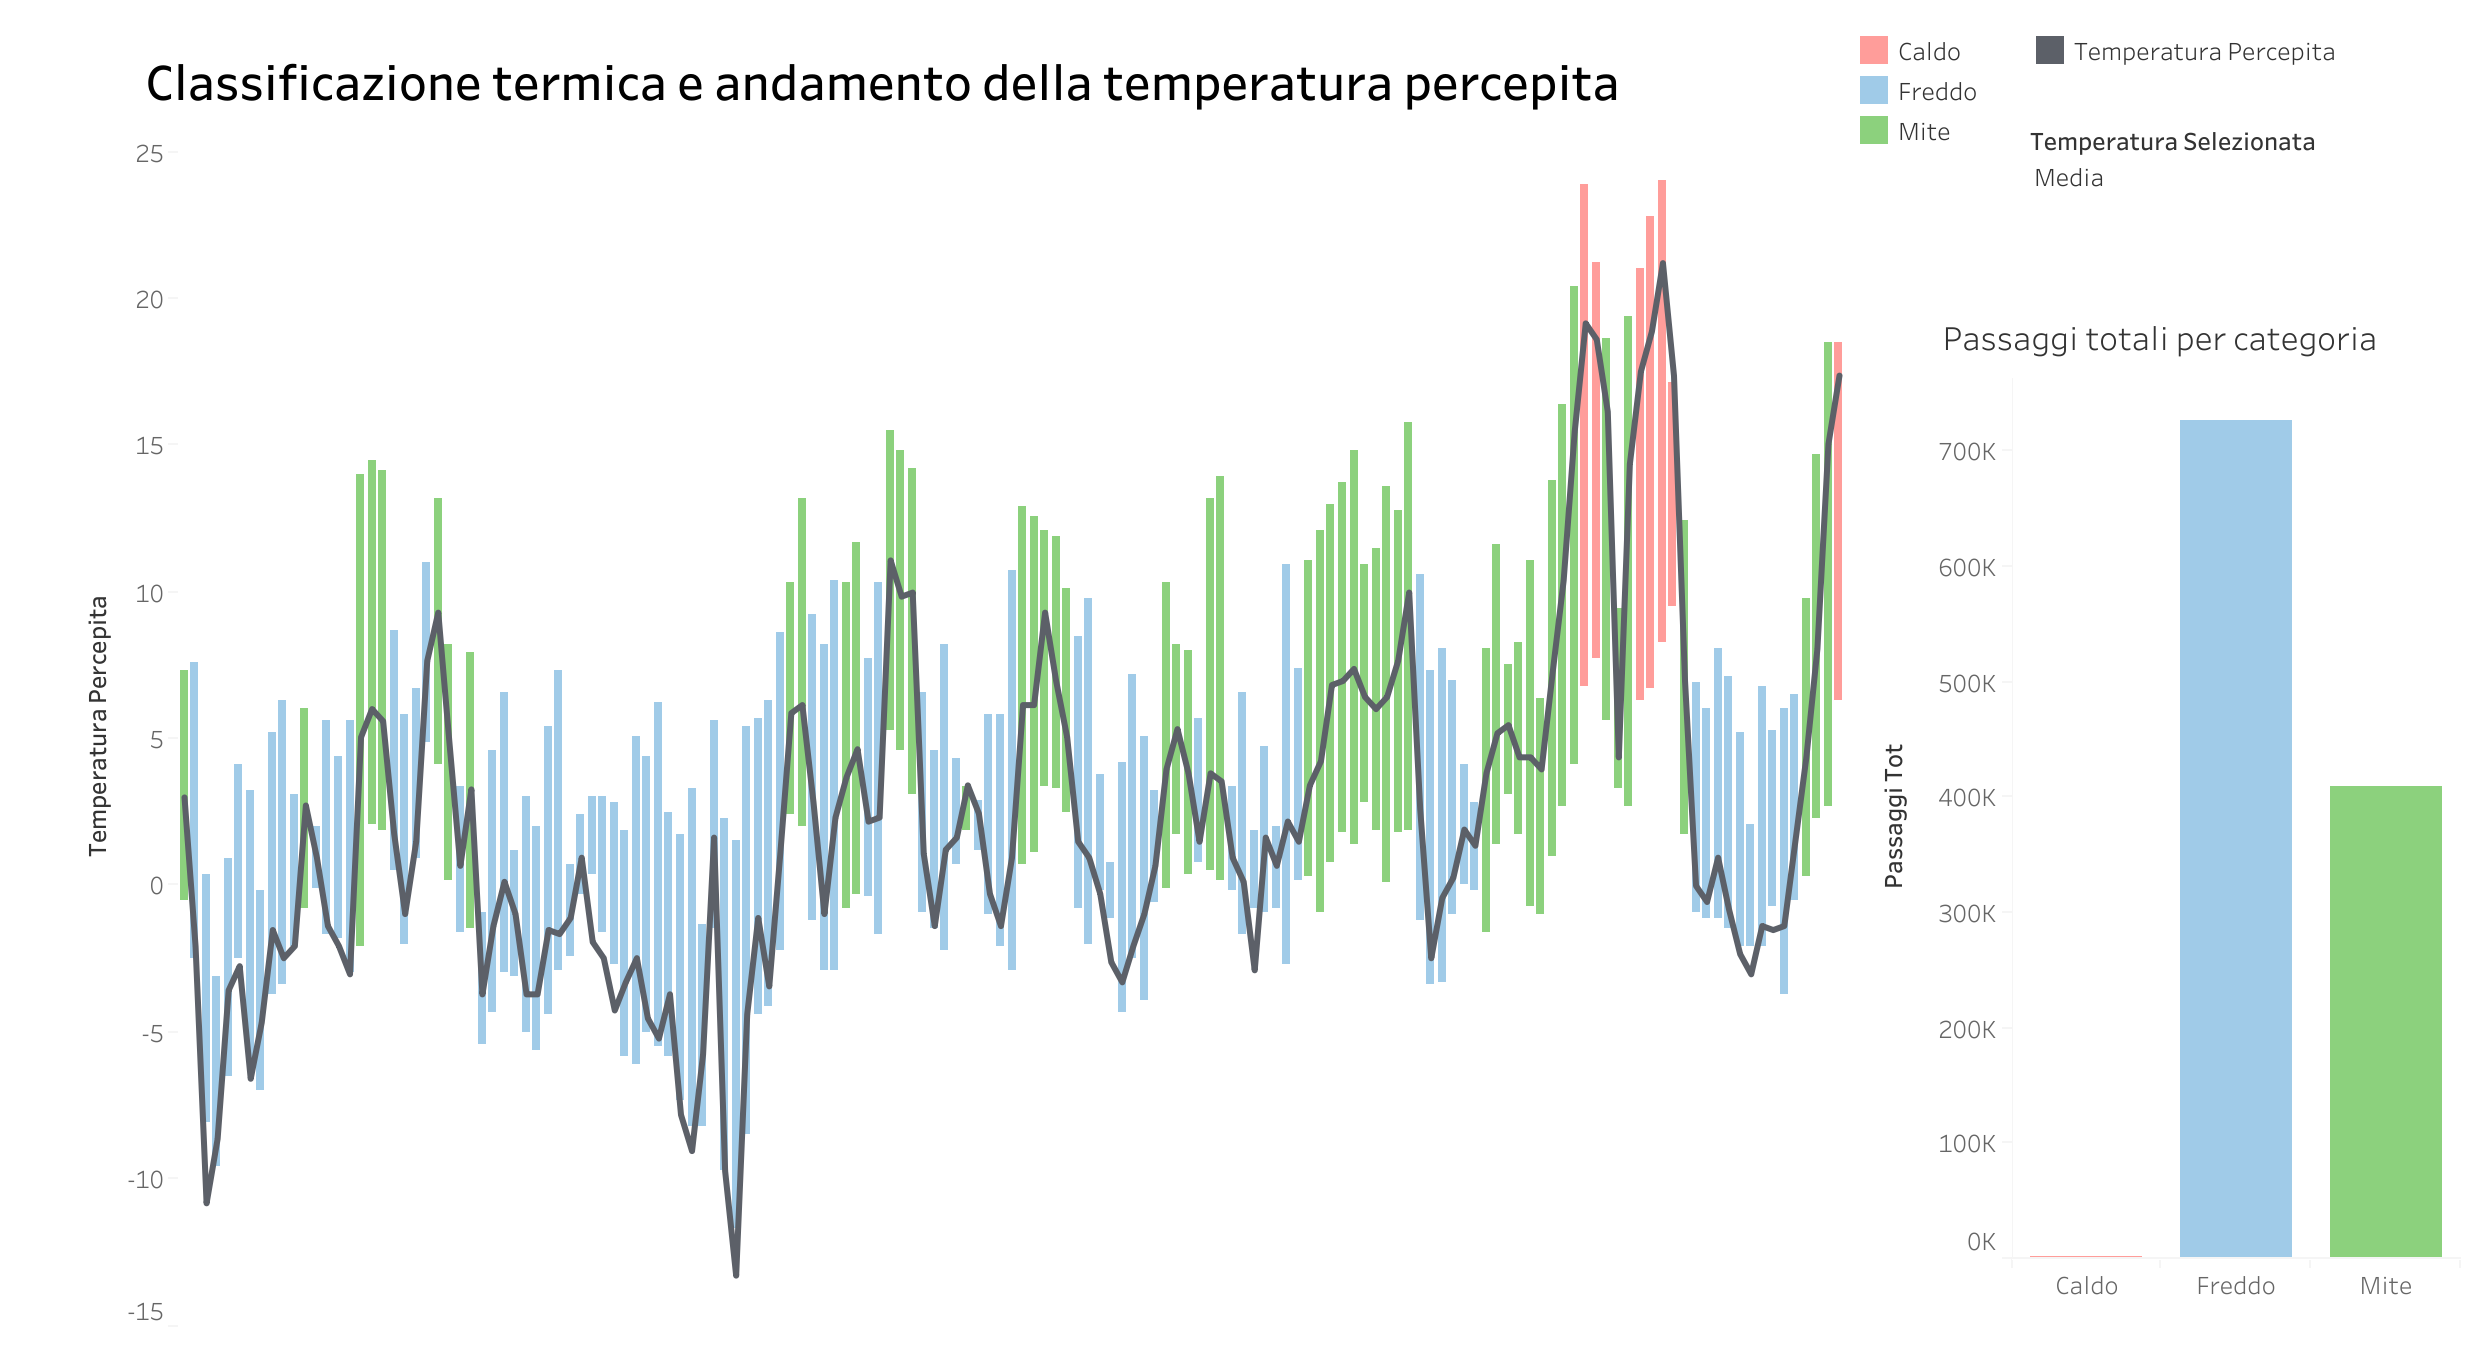
\includegraphics[width=0.95\textwidth]{images/Tableau/Studio_3/Classificazione Termica.png}
    \caption{Dashboard di classificazione termica e andamento della temperatura percepita}
    \label{fig:Classificazione termica}
\end{figure}



\paragraph{Struttura della visualizzazione e variabili impiegate}
\begin{itemize}
    \item \textbf{Asse X}: nella vista principale l’asse delle ascisse rappresenta le \textbf{date} dell’intera stagione, consentendo di associare ogni valore al relativo giorno di rilevazione. Nella vista secondaria, invece, l’asse X riporta le \textbf{categorie di temperatura} (\textit{freddo}, \textit{mite}, \textit{caldo}).
    
    \item \textbf{Asse Y}: nella vista principale viene impiegato un \textbf{doppio asse}. Il primo visualizza la \textbf{temperatura minima} e il parametro \textbf{Range Size}, che genera le barre verticali sospese e rappresenta l’escursione termica giornaliera. Il secondo asse mostra la \textbf{temperatura percepita}, rappresentata da una linea grigia sovrapposta alle barre.
    
    \item \textbf{Filtri e colorazioni}: ogni categoria termica è associata a un colore distinto (freddo = blu, mite = verde, caldo = rosso), mentre la linea della temperatura percepita è grigia per garantire contrasto e leggibilità. È inoltre presente un \textbf{parametro interattivo} che consente di modificare la base di calcolo della temperatura, scegliendo tra temperatura media (impostazione predefinita) e temperatura minima (vedi Appendice~\ref{appendix:Temp_Base}).
    
    \item \textbf{Tipologia di grafico}: combinazione a \textbf{doppio asse} costituita da barre verticali e linea continua, integrata da una vista secondaria a barre semplici per la distribuzione dei passaggi totali per categoria di temperatura.
\end{itemize}


\paragraph{Valutazioni e osservazioni}

Questa dashboard consente di catalogare e analizzare tutte le giornate della stagione, fornendo una rappresentazione continua delle variazioni termiche e delle condizioni percepite.  
Osservata in combinazione con le altre visualizzazioni, permette di collocare ciascun giorno all’interno di una specifica categoria termica e di interpretarne il potenziale impatto sui flussi di affluenza.\\

Dall’andamento della temperatura percepita si osservano diversi picchi minimi particolarmente bassi, in alcuni casi accentuati dall’effetto del vento.  
La vista secondaria evidenzia come le giornate fredde non costituiscano un deterrente per la pratica sciistica: rappresentano infatti la quota maggiore di presenza, quasi il doppio rispetto ai giorni classificati come “miti”.  
Al contrario, le giornate “calde” risultano estremamente limitate, appena sette in tutta la stagione, concentrate nella fase finale.\\

Verso la conclusione della stagione si nota inoltre un progressivo aumento dell’escursione termica giornaliera. Questo fenomeno, pur non potendo essere direttamente correlato ai flussi orari di affluenza (non inclusi in questo studio), suggerisce una possibile influenza sulla qualità della neve nelle ore centrali della giornata, che tende a deteriorarsi più rapidamente rispetto alle prime ore del mattino.


%-----------------------------------------

\section{Analisi 4 – Impatto delle giornate nevose sulle tipologie di Skipass}
\label{sec:analisi4}

La quarta analisi integra i dati meteorologici  personalizzati forniti da \textbf{ARPA Veneto}, relativi alle giornate caratterizzate da precipitazioni nevose, con i dati sui passaggi ai tornelli suddivisi per tipologia di Skipass.  
L’obiettivo  è comprendere in che misura le condizioni meteorologiche, e in particolare la presenza di neve, incidano sull’affluenza agli impianti e sull’utilizzo delle diverse tipologie di titolo di accesso.
La dashboard realizzata presenta una vista principale e due viste di supporto interattive, tra loro collegate attraverso parametri e filtri comuni.\\

Nella \textbf{vista principale} viene mostrato l’andamento giornaliero dei passaggi ai tornelli durante l’intera stagione invernale. Le colonne corrispondenti alle giornate di neve sono evidenziate con una colorazione distinta, in modo da rendere immediatamente visibile la distribuzione e l’intensità dei passaggi in relazione agli eventi nevosi.  
Questa rappresentazione consente di individuare rapidamente se, e in che misura, le giornate con precipitazioni abbiano determinato variazioni significative nei flussi di utenza rispetto alle giornate senza neve.\\

Le \textbf{viste secondarie}, collocate nella parte destra della dashboard, forniscono una sintesi numerica e comparativa dell’analisi.  
La prima riporta il totale complessivo dei passaggi avvenuti in giornate con e senza neve, mentre la seconda mostra la media giornaliera dei passaggi nelle stesse condizioni.  
Queste visualizzazioni complementari offrono una lettura aggregata del fenomeno e risultano utili per verificare la coerenza e l'ampiezza dell'impatto meteorologico osservato nel grafico principale.\\


Tutti i grafici sono collegati dai filtri che consentono di selezionare la condizione meteorologica (assenza o presenza di neve), e dal selettore di tipologia skipass (DS, Valle o Totale), nell'immagine è selezionato il titolo \textbf{DS} (vedi appendice \ref{fig:Impatto_neve_Valle} per altra vista).
La modifica di un parametro determina quindi l'aggiornamento di tutte le viste. Le due viste di supporto sono inoltre connesse a un filtro di mensilità per mostrare totali e medie anche in relazione ai vari mesi della stagione.
Tale filtro non è applicato alla vista principale, poiché l'obiettivo di quest'ultima è evidenziare la distribuzione complessiva delle giornate nevose lungo l'intero arco stagionale.
Di seguito viene presentata la visualizzazione completa nella figura ~\ref{fig:Impatto_neve}.

\newpage


\begin{figure}[htbp]
    \centering
    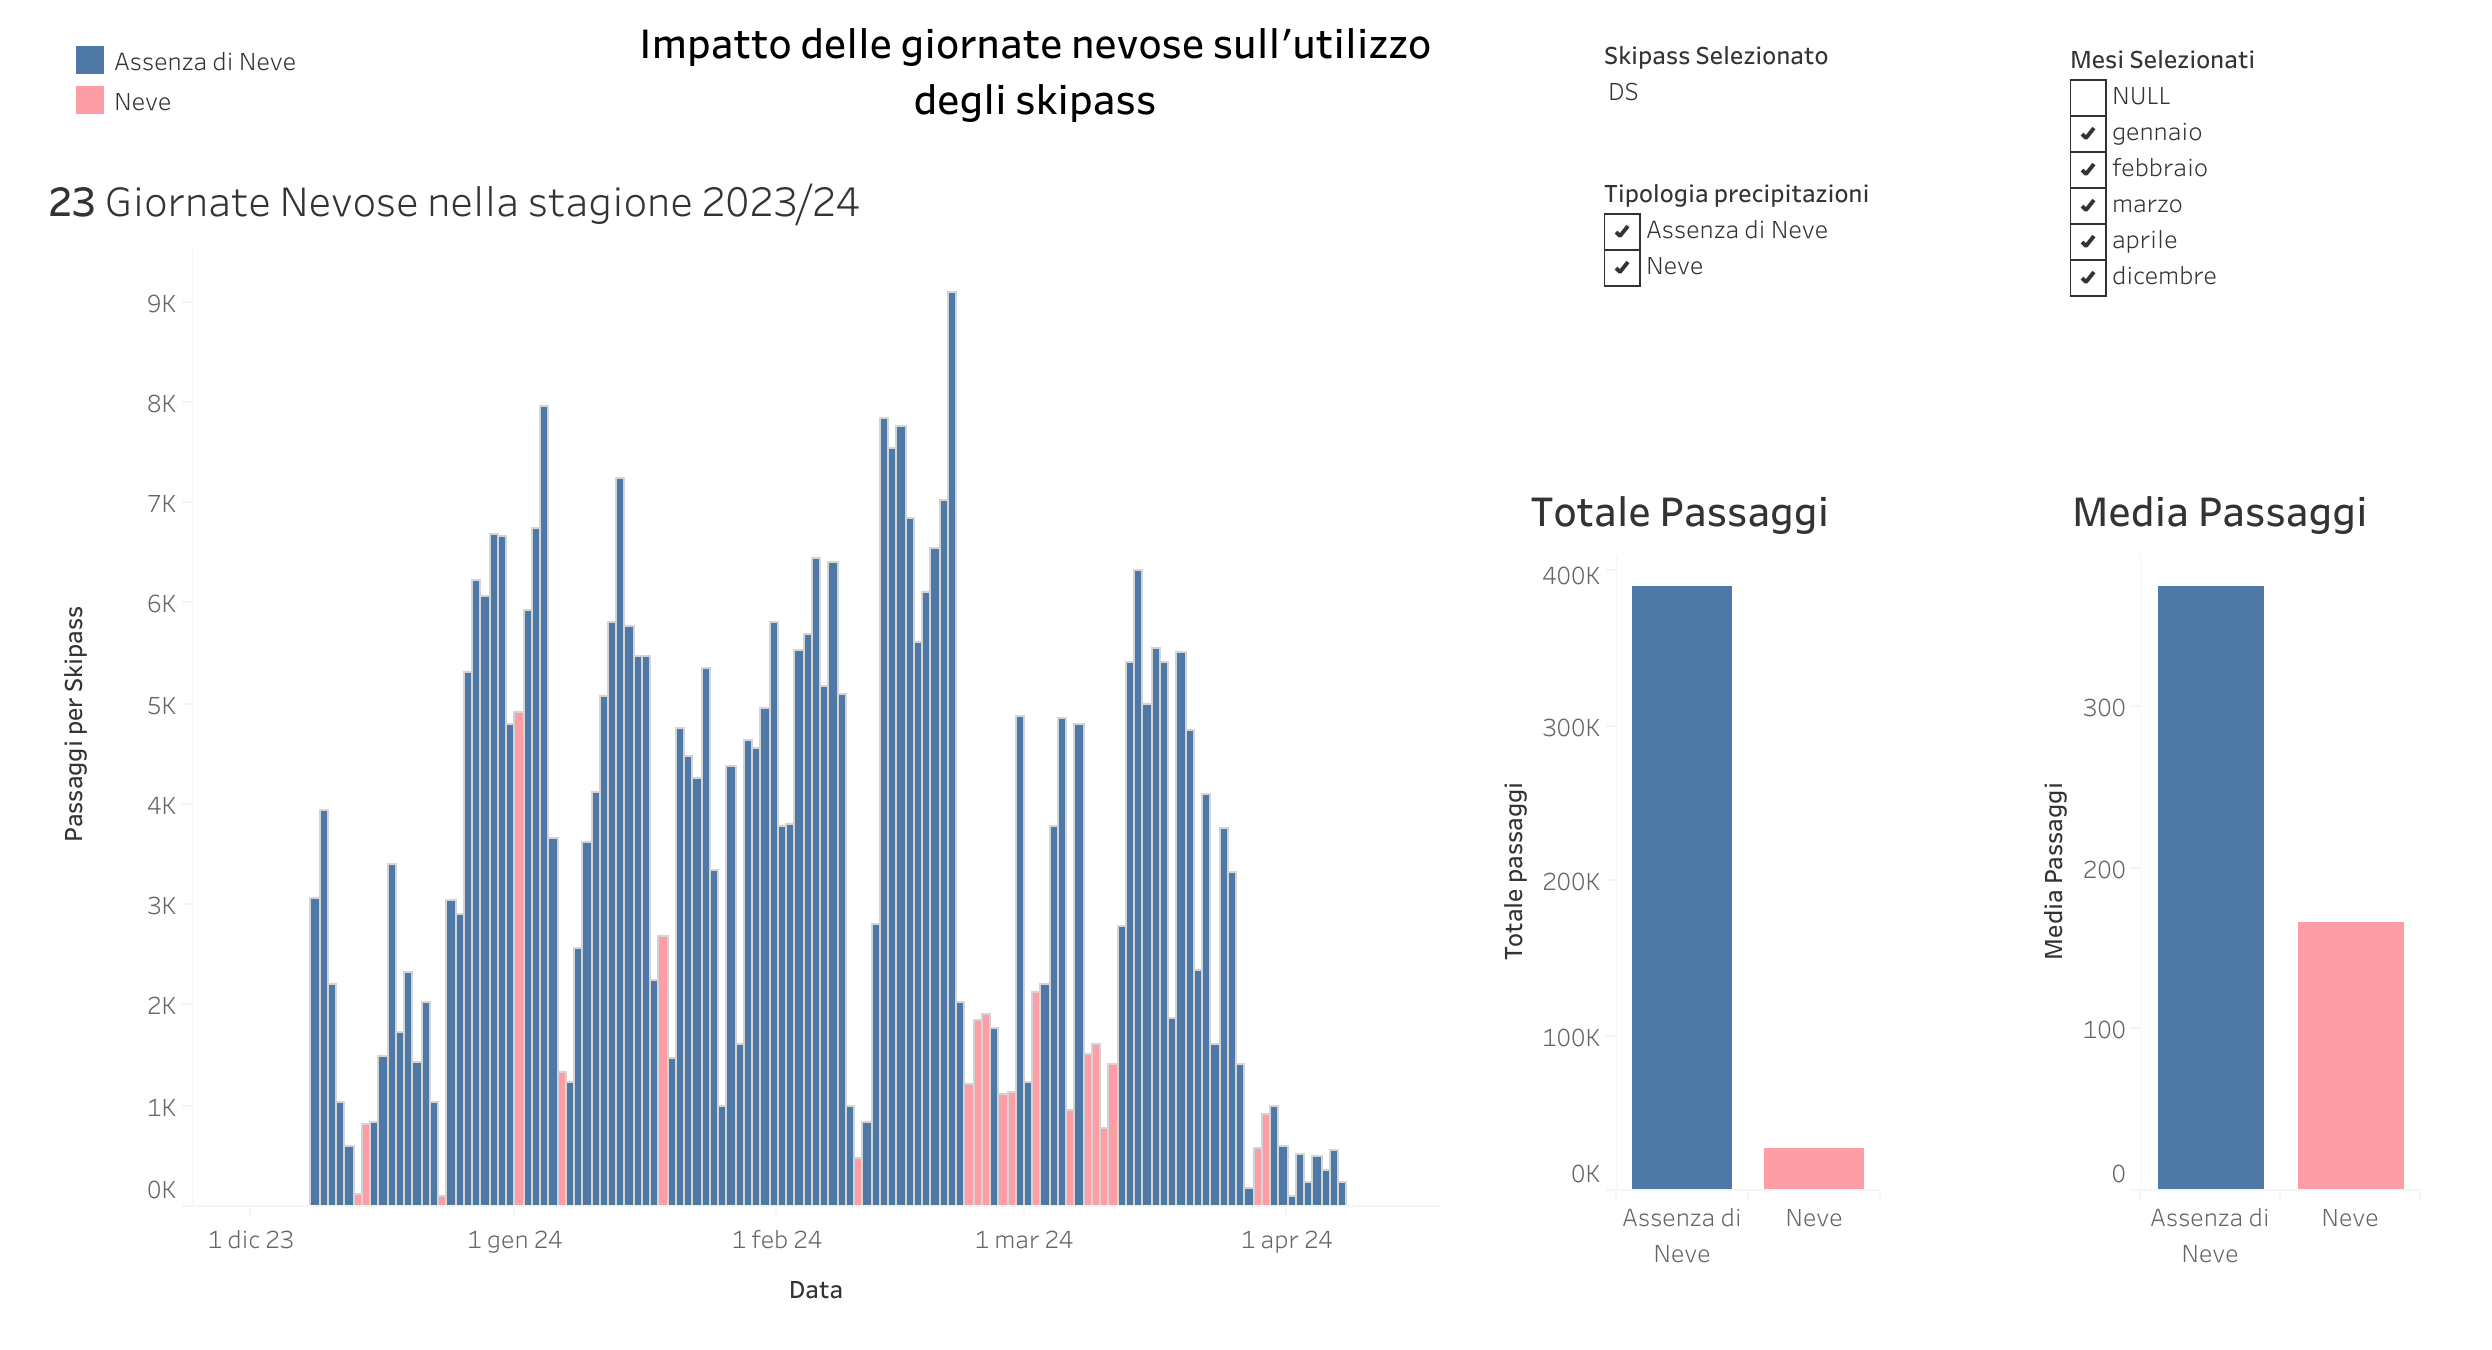
\includegraphics[width=0.95\textwidth]{images/Tableau/Studio_4/Impatto Neve.png}
    \caption{Dashboard Impatto giornate sull'utilizzo degli Skipass, vista Dolomiti Superski}
    \label{fig:Impatto_neve}
\end{figure}

\paragraph{Struttura della visualizzazione e variabili Impiegate}
\begin{itemize}
    \item \textbf{Asse X}: per la vista principale rappresenta la data (misura Continua); per le viste secondarie è invece impiegato il parametro \textbf{Neve} che distingue le date caratterizzate da una precipitazione nevosa (valore Neve), da quelle senza precipitazioni (valore Assenza di Neve)\footnote{Basato sui dati personalizzati forniti da ARPA \cite{ARPAV_private}.}.
    \item \textbf{Asse Y}: nella vista principale riporta il numero di passaggi in funzione della tipologia di skipass selezionata; nelle viste secondarie utilizza il medesimo parametro all’interno delle funzioni di aggregazione \textbf{Somma} e \textbf{Media}, rispettivamente per rappresentare i valori totali e medi giornalieri.
    \item \textbf{Filtri e colorazioni}: le colorazioni differenziano visivamente le giornate con neve (rosa) da quelle senza neve (blu); l’utente può scegliere se visualizzare entrambe o solo una delle due categorie. È inoltre presente un filtro a scelta singola per la tipologia di skipass basato sul parametro "Selezione Skipass" e, nelle viste secondarie, un filtro a scelta multipla che consente di selezionare i mesi da visualizzare.
    \item \textbf{Tipologia di grafico}: grafici a barre multiple, impiegate per entrambe le visualizzazioni.
\end{itemize}

\paragraph{Valutazioni e osservazioni}

Dall’analisi della vista principale e dei valori aggregati e medi giornalieri emerge che le giornate caratterizzate da precipitazioni nevose comportano una riduzione significativa dei passaggi complessivi agli impianti per entrambe le tipologie di skipass.
Tuttavia, l’intensità dell’impatto varia in modo sensibile: gli utenti dotati di \textbf{skipass Dolomiti Superski} registrano, nelle giornate con neve, un’affluenza pari a circa il \textbf{44\%} di quella osservata nelle giornate senza precipitazioni, mentre per gli utenti con \textbf{skipass Valle} tale valore si attesta intorno al \textbf{52\%} (Tabella~\ref{tab:Neve_medie}).

\begin{table}[h]
    \centering
    \begin{tabular}{lccc}
        \toprule
        \textbf{Tipo Skipass} & \textbf{Media Senza Neve} & \textbf{Media con Neve} & \textbf{Rapporto Neve/Assenza} \\
        \midrule
        Valle & 504,9 & 260,4 & 51,6\% \\
        DS & 374,4 & 165,9 & 44,3\% \\
        \bottomrule
    \end{tabular}
    \caption{\textbf{Medie giornaliere} di passaggi con e senza precipitazioni nevose, suddivise per tipologia di Skipass.}
    \label{tab:Neve_medie}
\end{table}


Questo andamento, in cui il titolo “DS” mostra una flessione più marcata rispetto al titolo “Valle”, è confermato anche dal confronto dei \textbf{passaggi totali}: il rapporto tra giornate con e senza precipitazioni nevose risulta infatti leggermente inferiore per lo skipass Dolomiti Superski (Tabella~\ref{tab:Neve_totali}), confermando una maggiore sensibilità di questa categoria di utenza alle condizioni meteorologiche.

\begin{table}[h]
    \centering
    \begin{tabular}{lccc}
        \toprule
        \textbf{Tipo Skipass} & \textbf{Passaggi Senza Neve} & \textbf{Passaggi con Neve} & \textbf{Rapporto Neve/Assenza} \\
        \midrule
        Valle & 526.056 & 43.232 & 8,2\% \\
        DS & 390.099 & 27.539 & 7,1\% \\
        \bottomrule
    \end{tabular}
    \caption{\textbf{Passaggi totali} con e senza precipitazioni nevose, suddivisi per tipologia di Skipass.}
    \label{tab:Neve_totali}
\end{table}


Questa differenza suggerisce che la presenza di neve influenzi in misura maggiore i flussi di sciatori  detentori di skipass DS, spesso non locali o provenienti da altri comprensori, verosimilmente a causa delle difficoltà di spostamento o delle peggiori condizioni di visibilità.
Al contrario, gli utenti titolari di \textbf{skipass Valle}mostrano un comportamento più stabile, confermando una maggiore propensione a frequentare gli impianti anche in condizioni meteorologiche avverse.
Tale tendenza potrebbe inoltre essere ricondotta alla diversa modalità di utilizzo dei titoli di accesso: gli sciatori in possesso di \textbf{skipass Dolomiti Superski} tendono più spesso a disporre di abbonamenti stagionali, che consentono una maggiore flessibilità nella scelta delle giornate di sci, mentre chi acquista uno \textbf{skipass Valle} spesso lo fa per periodi più brevi, ed è quindi generalmente più incline a sfruttare appieno il proprio acquisto, anche in presenza di condizioni meteo meno favorevoli.\\

In sintesi, la neve rappresenta un fattore limitante per l’affluenza complessiva, ma il suo effetto è modulato dalla tipologia di utenza e dal tipo di titolo di accesso utilizzato.\footnote{\textbf{Nota:} Per una vista complessiva delle 4 dashboard principali presentate in questo capitolo si veda l'appendice nella figura \ref{fig:vista_completa}.
Inoltre l'intero materiale è disponibile sul sito di Tableau Public visitabile inquadrando il QR code presente nella figura \ref{fig:qr_tableau} all'interno dell'appendice}


%-----------------------------------------
